\documentclass[conference]{IEEEtran}
\IEEEoverridecommandlockouts
% The preceding line is only needed to identify funding in the first footnote. If that is unneeded, please comment it out.
\usepackage{cite}
\usepackage{amsmath,amssymb,amsfonts}
\usepackage{algorithmic}
\usepackage{graphicx}
\usepackage{textcomp}
\usepackage{xcolor}
\def\BibTeX{{\rm B\kern-.05em{\sc i\kern-.025em b}\kern-.08em
    T\kern-.1667em\lower.7ex\hbox{E}\kern-.125emX}}

\usepackage[parfill]{parskip}


\setlength{\parindent}{0pt}
\newcommand{\forceindent}{\leavevmode{\parindent=1em\indent}}

%\usepackage{indentfirst}

\usepackage{url}

\def\IEEEkeywordsname{Keywords}

\begin{document}

\title{Differences between Embedded System Operating Systems and Mobile Operating Systems\\
%{\footnotesize \textsuperscript{*}Note: Sub-titles are not captured in Xplore and
%should not be used}
%\thanks{Identify applicable funding agency here. If none, delete this.}
}


\author{\IEEEauthorblockN{Wesly Yii}
\IEEEauthorblockA{\textit{BSc (Hons) in Computer Science} \\
%https://university.sunway.edu.my/tech/bsc-comp-sc
\textit{Sunway University}\\
Selangor, Malaysia\\
18066233@imail.sunway.edu.my}
\and
\IEEEauthorblockN{Tan Chun Ze}
\IEEEauthorblockA{\textit{Bachelor of Software Engineering (Hons)} \\
%https://university.sunway.edu.my/tech/bsc-software-eng
\textit{Sunway University}\\
Selangor, Malaysia\\
15020605@imail.sunway.edu.my}
\and
\IEEEauthorblockN{Lee Ming Zhen}
\IEEEauthorblockA{\textit{Bachelor of Software Engineering (Hons)} \\
\textit{Sunway University}\\
Selangor, Malaysia\\
18088757@imail.sunway.edu.my}
\and
\IEEEauthorblockN{Ryan Aung Yi Yang}
\IEEEauthorblockA{\textit{BSc (Hons) Computer Networking and Security} \\
%https://university.sunway.edu.my/tech/bsc-network-security
%course name too long so truncated some part of it
\textit{Sunway University}\\
Selangor, Malaysia\\
18007906@imail.sunway.edu.my}
}


\maketitle

\begin{abstract}
%This document is a model and instructions for \LaTeX.
%This and the IEEEtran.cls file define the components of your paper [title, text, heads, etc.]. *CRITICAL: Do Not Use Symbols, Special Characters, Footnotes, 
%or Math in Paper Title or Abstract.
Operating systems play a significant role in powering devices worldwide, this document seeks to provide a comparison between Embedded system operating systems and Mobile Operating systems.
\end{abstract}
\mbox{} \\
\forceindent \begin{IEEEkeywords}
embedded systems, mobile operating systems, operating systems, difference, compare
\end{IEEEkeywords}

\section{Introduction}
\forceindent Human activity is increasingly augmented with computing systems, and the hardware they run on usually have some kind of operating system on it, be it the phones in our pockets that use a Mobile Operating System, or the Subway ticket door that uses an Embedded system operating system.

%\bigskip
\forceindent In this document, we seek to provide a glimpse into the world of these two types of operating systems, by talking about each of their relevance, usage scenarios, pros and cons. We will also provide a brief comparison between Microkernel and monolithic kernel.

\section{Background}
\subsection{Embedded System Operating Systems}

\paragraph{What is it about?}\mbox{} \\
\forceindent Embedded system operating system is a type of operating system that carries out distinct processes for particular devices in order for them to operate optimally. It is just like a toned down version of a standard computer OS with limited functionality\cite{TNEOS}. Embedded system operating systems may exist as a standalone independent system or belong as a part of something bigger\cite{ITEOSMC}. \\

\\
\paragraph{Why the need for it?}\mbox{} \\
\forceindent The main reason for embedded OS to exist is to act as a partitioning tool as well as manage hardware and software resources for the embedded system to work as intended. It also simplifies software development in the upper layer by providing an abstraction layer. The need for it lies in how embedded operating systems can perform a dedicated function for a specific device to run while also allow it to be less demanding in terms of resource consumption\cite{ITEOSPV}.

\\
%\bigskip
\paragraph{What is the application?}\mbox{} \\
\forceindent Applications of embedded system OS include Embedded Linux, iOS, Windows Mobile OS, Blackberry OS, and Symbian. A Linux operating system that is utilized within embedded devices and appliances is called Embedded Linux. ATM machines utilising Windows XP is also an application of embedded operating systems.

\subsection{Mobile Operating Systems}\\
\paragraph{What is it about?}\mbox{} \\
\forceindent A mobile OS is another type of operating system that is created for the sole purpose of powering mobile devices. These mobile devices include PDAs, tablets, smartphones etc. Similar to how the Windows operating system works in a desktop, a mobile operating system allows different kinds of applications to run on a mobile device by serving as a software platform beneath the apps.
\\
\paragraph{Why the need for it?}\mbox{} \\
\forceindent A mobile operating system is essential for mobile devices to run ideally. A mobile operating system would enable multitasking, which means that multiple applications can run at one time. It will also allow the users to adjust the brightness and volume of all the applications through a single button. Other than that, applications would then be compatible and portable across multiple devices of different brands.
\\
\paragraph{What is the application?}\mbox{} \\
\forceindent Some notable examples of mobile OS are Apple’s iOS and Google’s Android OS. The differences between iOS and Android is that iOS is designed to only run on Apple devices within its XNU kernel while Android is an open source software which implies that it can be used by other mobile device manufacturers who are then able to customize the Android source code to fit their own device’s needs. Apple has also released other mobile OS meant for their Apple watch and iPad which is watchOS and iPadOS respectively\cite{CSMOS}.


\forceindent Covering all types of operating systems in embedded systems and mobile systems can be vague and challenging. With that said, Operating  systems  that are ubiquitous will be chosen to elaborate more in depth about their structure and features.



\section{In-depth review and discussion}


%\begin{center}
%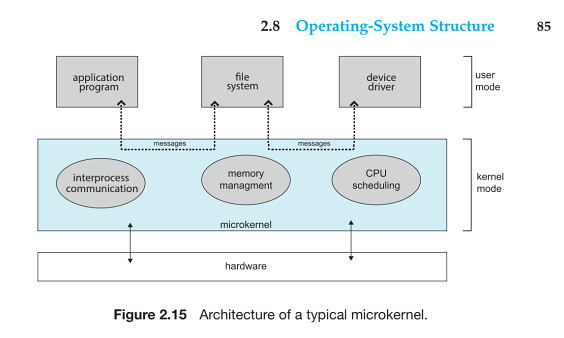
\includegraphics[scale=0.4]{./images/QNX_OS.png}
%\end{center}

%\subsection{Reason for using Microkernel in QNX}
%%\subsection{Efficiency}
%\paragraph{Efficiency}\mbox{} \\
%Microkernels require less resources to operate as they only contain essential functions(which are interprocess communication, memory management and CPU scheduling) to operate, it allows handling process and memory management to be more efficient. [1] With the benefits of minimal requirement of resources reduce the cost of building embedded systems.
%\\
%\subsection{Extentability}
%\paragraph{Extentability}\mbox{} \\
%%\paragraph{}
%Any services can be implemented easily in the user mode without affecting the kernel mode[1]. As a result, any services that need to be updated or modified can be done easily.
%\\
%%\subsection{Security and Reliability}
%\paragraph{Security and reliability}\mbox{} \\
%%\paragraph{}
%The kernel space will not be affected if any of the services is damaged, because services are only implemented in user mode instead of kernel mode according to SILBERSCHATZ.et al[1]. Damaged kernels can cause serious issues during real-time scenarios. For instance, failure of an anti-lock braking system causing severe accidents that will lead to high chances of deaths. Therefore, security and reliability is crucial to the real-time operating systems.

\paragraph{Microkernel in QNX Architecture} \mbox{} \\
\forceindent QNX is one of the operating systems used in real-time embedded systems. QNX heavily relies on Microkernel architecture to support its own operating system\cite{Burger}\cite{Galvinbook}.
%TODO: yet add page number for Galvinbook

%\subsection{QNX operating system}


\begin{figure}[h]
\caption{QNX Microkernel model}
\begin{center}
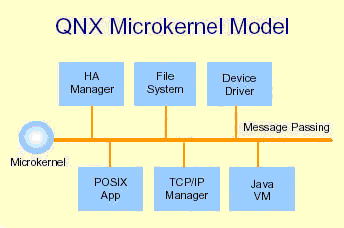
\includegraphics[scale=0.5]{./images/QNX_microkernel_mode.png}
\end{center}
\end{figure}

%\paragraph{}
\forceindent Microkernel only provides fundamental OS services including interprocess communication(IPC), memory management and CPU scheduling\cite{Galvinbook}. Other services are implemented as user-level programs located in separate address space from Microkernel\cite{Galvinbook}. To achieve extensible service implementation and communication between other services and microkernels. IPC is an important function as it uses message passing\cite{Burger} allowing other services to exchange messages between each other indirectly.

%\bigskip
\paragraph{Linux kernel in Android architecture} \mbox{} \\
\forceindent Android OS has a 86.1\% market share in the mobile OS market \cite{SMS}. It is based on the Linux kernel with a monolithic structure.

\begin{figure}[h]
  \caption{Android architecture}
\begin{center}
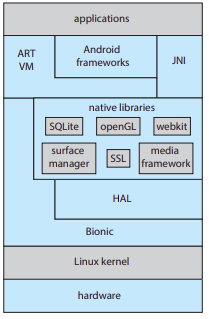
\includegraphics[scale=0.5]{./images/Android_architecture.png}
\end{center}
\end{figure}

%[1] again ffs, assume it is [A] so it Galvinbook
\forceindent Fundamental OS services and other non-essential services are combined together into one single address space\cite{Galvinbook}. System calls are used in android architect to allow application programs to interact with the kernel\cite{TDDBM}.

\forceindent Figure 2 indicates that android’s architecture consists of a layered stack of software providing an abundance set of frameworks and libraries to support crucial hardware features including graphics, audio\cite{Galvinbook}. For that reason, it gives the android operating system to be compatible with any types of android enabled devices.

\forceindent With the accumulated resources gathered, it can be concluded that embedded OS and mobile OS use different approaches on OS structure for different benefits, and using the wrong OS type could be devastating. Thus, the pros and cons of embedded operating system and mobile operating system shall be explained to aid the choosing of OS architectures.

%\bigskip
\subsection{Pros of Embedded OS}
\paragraph{Loads faster and consumes less power} \mbox{} \\
\forceindent Embedded system OS can be attached to a PC and will always load faster from the flash compared to a standard computer OS because of the limited features built in it. This is beneficial when users only need to perform a single task such as browsing the internet.\cite{TDDBM}

\paragraph{Distinct functions} \mbox{} \\
\forceindent Embedded system OS differs greatly from standard OS in terms of their abilities to perform different functions. Embedded OS will be limited to one single task and will perform the task regardless of user intervention. Examples of devices using an embedded OS would range from a simple toaster to specific embedded systems such as the QNX4 RIOS\cite{NOSvsEOS}.

\subsection{Cons of Embedded OS}
\paragraph{Hardly Scalable} \mbox{} \\
\forceindent Embedded system OS are usually not upgradable since it's system stays fixed after the initial configuration. Some embedded systems OS like the ones in  ATM machines are also designed to not receive upgrades to prevent tampering. Embedded system OS only allows upgrades if the chip is flashable. An example of an upgradable embedded system OS would be the one in a wifi router, it can be updated by flashing the card in the router upon downloading the new firmware\cite{lifewire}.

\subsection{Pros of Mobile OS}
\paragraph{Open source platforms are constantly updated and well-supported} \mbox{} \\
\forceindent Mobile  system OS such as Android open source software is one of the most widely used Mobile OS in the world.It is utilised by top mobile conglomerates like Huawei and Samsung. In recent years, we could see that there are more variations of the open source platform to support and cater to specific markets like the HongMengOS (Harmony OS) that is launched in 2019 for new Huawei devices exclusively\cite{HuaweiHongmeng}. Such new launches suggest that Mobile system OS are still in high demand and will be the focal point of operating systems in many years to come.

\paragraph{Convenience and flexibility} \mbox{} \\
\forceindent Mobile  system OS is a newer concept and is built to focus on being convenient to its users. It is improved on existing OS and opts to strive in responsive design, consistent and stable network access and possible improvements to be used in the diverse wireless environment\cite{technopedia}.

Mobile system OS like Android are open-source and are widely used as a base for many relatable OS like HarmonyOS. The fact that it is open source opens itself to many possibilities. It is flexible because many others improve and adjust the software to cater to their own needs.

\subsection{Cons of Mobile OS}
\paragraph{Instability} \mbox{} \\
\forceindent Mobile system OS struggles with the constraints of handling constant cellular interruptions and communications, power issues and the load on handling multiple applications launched by the user\cite{AAWP}. On average, a mobile phone easily uses anywhere from 50 to 500 processes on a comparatively smaller capacity compared to an embedded system OS which commonly runs a single shell. This leads to frequent crashes and bugs that leads to complications and instabilities.

\paragraph{Battery / Power} \mbox{} \\
\forceindent Mobile OS runs on a limited battery capacity unlike embedded OS which runs with a constant power supply. Although modern mobile devices now are equipped with better batteries, they are still lacking and unable to keep up with improvements in graphics and animations like in triple A games for mobiles. Many background processes are also capable of draining the battery, accelerating its wear.

\section{Conclusion}
\forceindent After looking into both embedded system OS and mobile OS, we can see that both types of OS have their own pros and cons. However, in terms of efficiency in performing what they are meant to do, QNX microkernel architecture is by far the most superior. Being small in size,it provides complete memory protection as it runs in the kernel space while other processes run in the user space. Most importantly, we think QNX is a good fit here as it is the best for mission critical applications due to the fact it never crashes thus making it robust, as any third party crashes does not impact the kernel itself and it keeps running at all times\cite{quora}.

%\section*{Acknowledgment}
%The preferred spelling of the word ``acknowledgment'' in America is without 
%an ``e'' after the ``g''. Avoid the stilted expression ``one of us (R. B. 
%G.) thanks $\ldots$''. Instead, try ``R. B. G. thanks$\ldots$''. Put sponsor 
%acknowledgments in the unnumbered footnote on the first page.

%\section*{References}
\bibliographystyle{IEEEtran}
%\bibliography{bib}
%\bibliography{IEEEexample}
\bibliography{mainbib}


\end{document}
